\chapter{Verification and code inspection}\label{ch:c8}\label{ch:verification}
This chapter reports how the coupling was tested. Nine complementary approaches were used
(Table~\ref{tab:vapproach}).

\begin{plain}
Before anyone relies on a model, it must be shown to be right. The coupling was tested in several independent ways:
automatic checks that no water is created or lost, comparisons with exact textbook solutions, comparisons with independent
software, hundreds of random test set-ups, and a line-by-line reading of the code.
\end{plain}

\begin{table}[!htbp]\centering
\caption{Verification approaches.}\label{tab:vapproach}
\begin{tabularx}{\linewidth}{P{0.27\linewidth}Y P{0.13\linewidth}}\toprule\hdr
Approach & What it shows & Section\\\midrule
Regression against Raven 4.15 & models without groundwater give identical results & \ref{sec:regression}\\
Automated audit of every run & exact water accounting on both sides; MODFLOW's balance & \ref{sec:audit}\\
Behaviour tests & pumping, drying, restarts, ensembles and every exchange behave as expected & \ref{sec:behaviour}\\
Grid types & geometry, format cross-checks, analytical solution, restarts and randomized tests for every grid & \ref{sec:vgrids}\\
Existing model & projections, units, round trip, overlap weights, restarts, safeguards, randomized tests & \ref{sec:vexisting}\\
Independent checks & geometry against standard libraries; flows against MODFLOW's own budget; grid and time-step invariance; faulty input & \ref{sec:independent}\\
Randomized testing & hundreds of random set-ups combining every option & \ref{sec:fuzz}\\
Code inspection & line-by-line reading, compiler, static analysis, memory and undefined-behaviour sanitizers & \ref{sec:codeaudit}\\\bottomrule
\end{tabularx}
\end{table}

Models without
groundwater were run with the unmodified Raven~4.15 and with the coupled code, both built with NetCDF:
\begin{itemize}
\item the Liard model: all outputs identical byte for byte;
\item the benchmark models distributed with Raven (\cmd{benchmarking/\_InputFiles}): the eleven that run give identical
      outputs, except that Lake of the Woods, whose reservoir in basin~44 dries out on 45 days, books less evaporation on
      those days. Its hydrographs and reservoir stages are identical; its
      cumulative balance error falls from 5.44 to 4.97~mm, and its \cmd{solution.rvc} carries the reservoir stages with 12
      digits. The other fourteen benchmark set-ups stop with the same input error in both builds (a missing \cmd{.rvt} file,
      wilting point above field capacity), as they do in the unmodified Raven~4.15.
\end{itemize}
The changes made to Raven itself affect only ensembles, reservoirs with absolute stages or
that dry out, restart files, constituent observations and the \cmd{:rvg\_Filename} command.

\section{Automated audit of every run}\label{sec:audit}
The tool \cmd{tools\_audit.py}, shipped with the example, checks any output folder for:
\begin{enumerate}
\item \textbf{recharge:} $\left(\sum V^{\mathrm{Raven}}-\sum V^{\mathrm{MF6}}-\Delta V^{\mathrm{dl}}-\sum V^{\mathrm{CHD}}\right)/\sum V^{\mathrm{Raven}}$;
\item \textbf{MODFLOW's balance:} cumulative imbalance relative to the gross flow, and the worst single step;
\item \textbf{convergence:} steps that failed to converge;
\item \textbf{seepage, rivers and surface stores:} the volume applied to Raven against MODFLOW's flow, including carried river losses;
\item \textbf{reservoirs:} the seepage sent to MODFLOW each step against the volume that left the lake the step before, and
      the volume MODFLOW took against the volume sent;
\item \textbf{Raven's balance:} the largest mass-balance error in \cmd{Watershed\allowbreak Storage.csv};
\item \textbf{outputs:} finite heads, contiguous end-of-step dates, a $t=0$ row for monitoring wells.
\end{enumerate}
Table~\ref{tab:audit} gives the results. The 20-year Liard run gives outputs identical to those runs, and the reservoir and ensemble runs were repeated
(Section~\ref{sec:behaviour}).

\begin{table}[!htbp]\centering
\caption{Relative errors are shares of the water moved. In every run the seepage returned to Raven equals MODFLOW\textquotesingle s seepage exactly, the surface-store bookkeeping is exact, no river loss is carried at the end and the output dates are contiguous. The one failed step is the rewetting day of the deliberately extreme drying test (Section~\ref{sec:behaviour}).}\label{tab:audit}
\footnotesize\setlength{\tabcolsep}{2.8pt}\begin{tabular}{lrrrrrrr}\toprule\hdr
Run & Steps & Recharge & \shortstack[r]{MODFLOW\\residual} & \shortstack[r]{Worst\\step [\%]} & \shortstack[r]{Failed\\steps} & River & \shortstack[r]{Raven\\balance [mm]}\\\midrule
20-year Liard & 7\,305 & 0 & $-1.0\times10^{-10}$ & $4.2\times10^{-6}$ & 0 & $1.1\times10^{-12}$ & 0.52\\
Pumping & 1\,826 & 0 & $-1.6\times10^{-10}$ & $7.1\times10^{-6}$ & 0 & $-9.6\times10^{-12}$ & 0.52\\
Fixed head, delay & 730 & $-3.2\times10^{-11}$ & $-3.9\times10^{-10}$ & $5.1\times10^{-6}$ & 0 & $7.7\times10^{-12}$ & 0.52\\
Restart & 365 & $-1.7\times10^{-11}$ & $-1.9\times10^{-10}$ & $3.2\times10^{-6}$ & 0 & $2.1\times10^{-11}$ & 0.06\\
Ensemble & 731 & 0 & $-1.7\times10^{-11}$ & $1.6\times10^{-7}$ & 0 & $9.5\times10^{-12}$ & 0.52\\
Wetlands & 730 & 0 & $-1.1\times10^{-10}$ & $1.5\times10^{-6}$ & 0 & $2.2\times10^{-11}$ & 0.52\\
Reservoir & 731 & 0 & $-1.7\times10^{-11}$ & $1.6\times10^{-7}$ & 0 & $9.5\times10^{-12}$ & 0.52\\
Soil-less HRUs & 365 & 0 & $-4.5\times10^{-11}$ & $7.4\times10^{-7}$ & 0 & $-1.2\times10^{-12}$ & 0.52\\
Drying (extreme) & 1\,826 & 0 & $-3.1\times10^{-4}$ & 43.2 & 1 & $8.1\times10^{-12}$ & 0.52\\
\bottomrule\end{tabular}\end{table}


\section{Behaviour tests}\label{sec:behaviour}
\begin{table}[!htbp]\centering
\caption{Behaviour tests.}\label{tab:behaviour}
\begin{tabularx}{\linewidth}{P{0.19\linewidth}P{0.27\linewidth}Y}\toprule\hdr
Test & Set-up & Result\\\midrule
Full Liard model & 20 years, 85 coupled HRUs, 3\,252 active columns & recharge exact; MODFLOW residual $10^{-10}$; no failed step; Raven balance 0.52 mm\\
Pumping & 100\,000 m$^3$/d well, 5 years & 93\% delivered; seasonal drawdown 0.8--8 m in the pumped cell, none 12 km away; 91--98\% of the water captured from rivers (Figure~\ref{fig:pumping})\\
Monitoring wells & synthetic heads with 5 cm noise & RMSE 4.9 cm; NSE 0.991--0.9997\\
Fixed-head lake & 9 cells & heads held exactly; recharge on them redistributed\\
Restart & 1 + 1 years against 2 years & flows within $6\times10^{-6}$ (Figure~\ref{fig:hotstart})\\
Ensembles & 2 Monte Carlo members, every option on & members identical to each other and to a single run\\
Drying and rewetting & valley aquifer starting dry & 26 wet areas merge into 2 and split with the seasons (Figure~\ref{fig:conn}); one rewetting step of 1\,826 does not converge and is flagged\\
Wetlands and lakes & 1\,903 exchange cells & water removed from Raven equals MODFLOW's leakage exactly\\
Reservoir & 50 km$^2$ lake on a coupled HRU & seepage delivered each day equals Raven's seepage of the day before\\
Soil-less HRUs & glacier HRUs coupled & seepage goes to surface water; balance unchanged\\
Other features & \cmd{:rvg\_Filename}, NetCDF, linkage cache, calibration & file found; NetCDF equals the binary heads within $10^{-4}$ m; cached run identical; DDS recovers gravel $K$ and $S_y$ within 5\%\\\bottomrule
\end{tabularx}
\end{table}


\begin{figure}[!htbp]\centering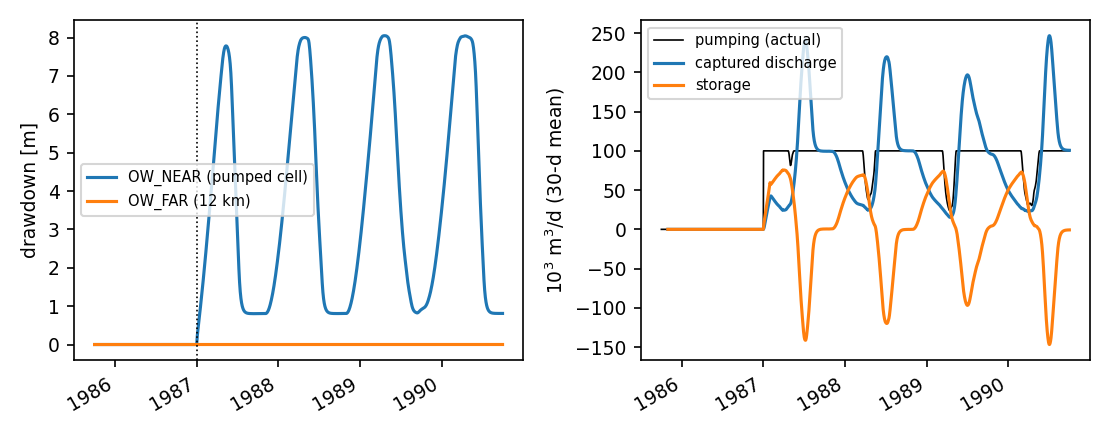
\includegraphics[width=\linewidth]{figures/fig_pumping.png}
\caption{Pumping test: drawdown at the monitoring wells (left) and where the pumped water comes from (right).}\label{fig:pumping}\end{figure}
\begin{figure}[!htbp]\centering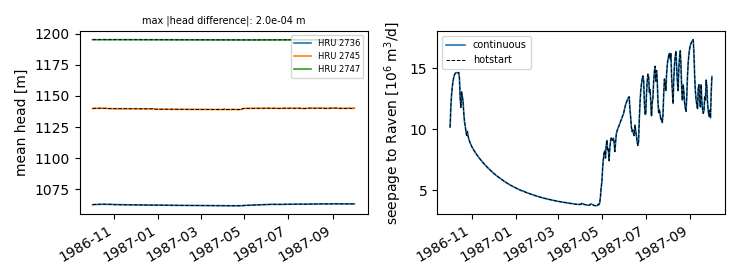
\includegraphics[width=\linewidth]{figures/fig_hotstart.png}
\caption{Restart: the second year of a continuous run (solid) and of a run restarted from \cmd{solution.rvc} (dashed).}\label{fig:hotstart}\end{figure}
\begin{figure}[!htbp]\centering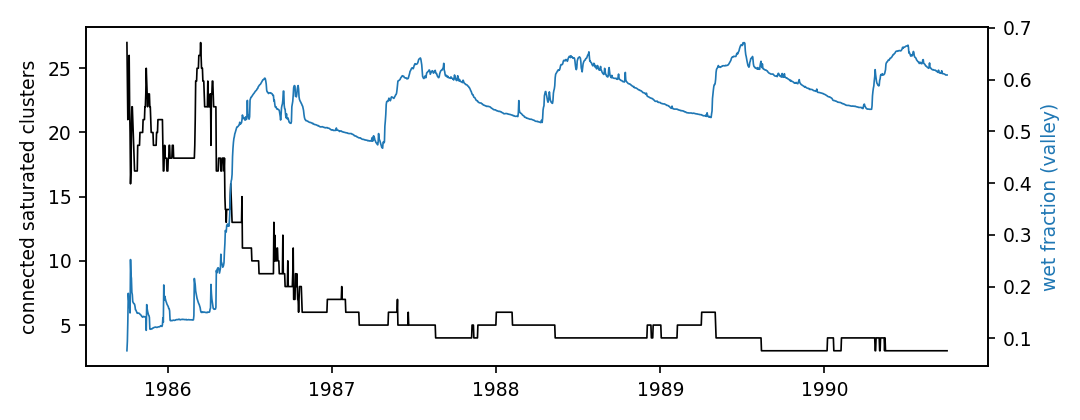
\includegraphics[width=0.9\linewidth]{figures/fig_connectivity.png}
\caption{Drying and rewetting: number of separate wet areas in the top layer (black) and wet fraction of the valley aquifer (blue).}\label{fig:conn}\end{figure}

\section{Independent checks}\label{sec:independent}
\subsection{Geometry against standard libraries}
The geometry functions were compiled into a stand-alone test and compared with widely used libraries (Table~\ref{tab:geom}).
\begin{table}[!htbp]\centering
\caption{Geometry functions against independent libraries.}\label{tab:geom}
\begin{tabularx}{\linewidth}{Y P{0.22\linewidth}P{0.2\linewidth}}\toprule\hdr
Function & Reference & Largest difference\\\midrule
Polygon clipping and area (400 random, mostly concave polygons) & shapely & $1.3\times10^{-10}$\\
Equal-area projection (300 points over the Liard region) & pyproj (same sphere) & $5\times10^{-7}$ m\\
Projection round trip & -- & exact\\
Bilinear raster sampling with a no-data cell (200 points) & independent code & $4\times10^{-7}$\\
GeoJSON and ASCII-grid variants (3-D coordinates, string IDs, holes, cell-centre headers, \dots) & shapely, reference values & read correctly\\\bottomrule
\end{tabularx}
\end{table}

\subsection{Exchanged flows against MODFLOW's own budget}
MODFLOW writes its own volume budget in its list file. For runs covering every package, every flow the coupling exchanged
was compared with MODFLOW's figure for the same step (Table~\ref{tab:listcheck}); the differences are at the printing
precision of the list file.
\begin{table}[!htbp]\centering
\caption{Coupler flows against MODFLOW's list-file budget.}\label{tab:listcheck}
\begin{tabularx}{\linewidth}{P{0.25\linewidth}Y P{0.2\linewidth}}\toprule\hdr
Run & Packages compared & Largest difference\\\midrule
20-year Liard & recharge, drains, rivers, storage & $6.2\times10^{-7}$\\
Pumping and boundaries & + wells, general-head boundaries & $6.9\times10^{-7}$\\
Fixed head and delay & + fixed heads & $6.1\times10^{-8}$\\
Wetland exchange & + store exchange & $1.1\times10^{-7}$\\
Reservoir & + reservoir seepage & $2.6\times10^{-7}$\\
Drying & + water-table ET & $4.1\times10^{-8}$\\\bottomrule
\end{tabularx}
\end{table}

\subsection{Grid size and time step}
The accounts stay exact for any cell size and time step (Table~\ref{tab:invariance}; subbasin 52, one year). These runs used
the earlier head tolerance of 0.01 m; the 0.47\% step on 4 km cells is what led to the present default of 0.00001 m.
\begin{table}[!htbp]\centering
\caption{Invariance to cell size and time step.}\label{tab:invariance}
\begin{tabular}{lrlrr}\toprule\hdr
Set-up & Active columns & Recharge & Worst step & Raven balance\\\midrule
1 km cells & 2\,147 & exact & 0.029\% & 0.456 mm\\
2 km cells & 545 & exact & 0.092\% & 0.456 mm\\
4 km cells & 142 & exact & 0.47\% & 0.456 mm\\
4 km cells, tighter tolerance & 142 & exact & 0.002\% & 0.456 mm\\
2 km cells, half-day steps & 545 & exact & 0.059\% & 0.219 mm\\\bottomrule
\end{tabular}
\end{table}

\subsection{Faulty input}
Thirty-nine faulty or unusual set-ups were run. Every error stops the run with a message that names the problem --- no crash
--- and every tolerated case runs (Table~\ref{tab:faulty}).
\begin{table}[!htbp]\centering
\caption{Response to faulty or unusual input.}\label{tab:faulty}
\begin{tabularx}{\linewidth}{Y P{0.4\linewidth}}\toprule\hdr
Input & Response\\\midrule
Missing HRU file or ID field; unknown profile or class; malformed class row & stops; names the file, field, profile or row\\
Aquiclude as top layer; zero layer thickness; value out of range ($K\le0$, $S_y>1$, negative delay, \dots) & stops; names the parameter\\
Process draining \cmd{GROUNDWATER} in a coupled HRU; no process feeding it & stops; names the process and HRU\\
Wrong library path; missing raster; well outside the model & stops; names the path, file or well\\
Duplicate IDs or names; two exchanges on one store; boundary without \cmd{HEAD} & stops; names the item\\
Malformed groundwater command in \cmd{.rvg}, \cmd{.rvt} or \cmd{.rvc} & stops; names the command\\
Hotstart heads for a different grid; cells larger than the HRUs & stops; explains the mismatch\\
Monitoring well outside the model; unknown \cmd{.rvg} command & runs with a warning\\
\cmd{TO\_BEDROCK} in a middle layer; no DEM or bedrock map; coupling switched off & runs as documented\\\bottomrule
\end{tabularx}
\end{table}

\section{Randomized testing}\label{sec:fuzz}
A test driver builds random but valid set-ups of the subbasin-52 model, drawing every option at random: cell size
(1--3 km), minimum coverage, one-day or half-day steps, conductivities, initial depth, seepage leakance and smoothing,
water-table ET, recharge delay, steady-state start, wetland exchange, 0--2 pumping wells, monitoring wells, a general-head
boundary, a fixed-head area and a coupled reservoir. Every run is checked independently of the audit tool: exact recharge,
seepage, river, store and reservoir identities; MODFLOW's balance (every converged step below 0.1\%, cumulative below
$10^{-4}$); Raven's balance below 1 mm; agreement with MODFLOW's list file; and, for about a third of the set-ups, a restart
that must reproduce the continuous run (every flow within $10^{-4}$ of its largest value in the run).

The code, with MODFLOW 6.8.1, passes the rounds that \cmd{tests/run\_all.py} repeats: 72 of 72 set-ups
over every grid type and 24 of 24 with a reservoir and lake refinement (Section~\ref{sec:vgrids}).

\section{Grid types}\label{sec:vgrids}
\begin{plain}
Every kind of grid was checked in four ways: its cells cover the area exactly with no gaps or overlaps; two different ways of
handing the same cells to MODFLOW give the same answer; the answer matches an exact textbook solution and gets closer to it
as the cells get smaller; and a restarted run matches a continuous one. Existing models are not affected by the new options.
\end{plain}
Every grid option was verified the same way as the default grid, plus four checks specific to grids.


\paragraph{Geometry of the grids.} A stand-alone test checks every generator: cells tile the domain exactly (area sums
equal to $10^{-15}$), neighbours are symmetric, each cell's perimeter equals its shared faces plus the domain edge, Voronoi
connections are exactly orthogonal, quadtree neighbours differ by one level at most, clipping handles concave cells and
lattices of cocircular seeds, and grids survive the linkage cache bit for bit.

\paragraph{Two formats, one answer.} The quadtree cells were run once as DISV (MODFLOW computes the geometry) and once
imported as DISU (the coupler computes connection lengths, face widths and directions): all flows agree to $6\times10^{-7}$ and
water tables to 0.3 mm. A regular grid written as DISU gives heads identical to DIS. Solving the coupler's DISU equations
independently in Python reproduces MODFLOW's heads to $3\times10^{-8}$ m.

\paragraph{Analytical solution.} A textbook case has an exact answer to compare with: a single well pumping from an aquifer
whose water level is held fixed all around, far away (the \emph{Thiem} solution). Close to the well the water level falls in
a known way with distance. A well pumping 5\,000 m$^3$/d from a confined aquifer ($T=500$ m$^2$/d) inside a
20 km square with fixed heads on its edge should give the Thiem profile $h=A+\frac{Q}{2\pi T}\ln r$. The slope fitted to
all cells between four cell sizes and 3 km from the well is compared with $Q/(2\pi T)$ in Table~\ref{tab:thiem}: every grid
converges to the analytical value as its cells shrink, and the solutions are symmetric around the well (slopes in the four
directions within 0.6\%).

\begin{table}[!htbp]\centering
\caption{Thiem test: error of the fitted slope $\partial h/\partial\ln r$.}\label{tab:thiem}
\begin{tabular}{lrrr}\toprule\hdr
Grid & Coarse & Medium & Fine\\\midrule
Regular, 500 / 250 / 125 m & +0.60\% & +0.04\% & +0.01\%\\
Regular 250 m, rotated 17\textdegree & & +0.03\% & \\
Regular 1 km refined to 125 m at the wells & & +1.01\% & \\
Quadtree, base 1\,000 / 500 / 250 m, 62.5 m at the wells & +0.80\% & +0.59\% & +0.26\%\\
Imported cells (the 250 m quadtree) & & & +0.25\%\\
HRU mesh, 500 / 250 m (250 m with XT3D) & +0.57\% & +0.29\% & $-$0.06\%\\\bottomrule
\end{tabular}
\end{table}

\paragraph{Lakes.} A reservoir with seepage to the aquifer was placed on the largest coupled HRU of subbasin~52 and each
refinable grid (3~km cells) was refined around it with \cmd{LAKES}. The median size of the cells touching the lake fell from
3\,000 to 750~m (rotated regular grid), from 3\,000 to 375~m (quadtree) and from 1\,210 to 490~m (HRU mesh); a
\cmd{POLYGONS} file with the same outline gives the same mesh. The water accounts stay exact (MODFLOW residual below
$1.2\times10^{-11}$), and the reservoir's seepage reaches MODFLOW exactly one step after it leaves the lake (sent $=$
previous step's volume in transit to $1.6\times10^{-10}$; delivered $=$ sent); MODFLOW's own list-file budget shows the same
reservoir seepage. Two randomized rounds --- 20 set-ups over all grid types and 12 that always have a reservoir and lake
refinement --- all passed every check, including the reservoir identity, which the
audit tool reports for every run with a reservoir; the rounds the test suite repeats are reported below.


\paragraph{Randomized testing.} The randomized set-ups of Section~\ref{sec:fuzz} were extended with a random grid (regular,
rotated and refined, quadtree, HRU mesh, imported cells, layers by elevation), random rotation, refinement and XT3D choice.
With this scale the largest deviation is $3.1\times10^{-6}$.

The two exceptions had
drawn the optional fully implicit XT3D: one failed to converge on 38 of 45 days (its accounts on the converged days are
exact; on the others the safeguard limits the exchange, as designed) and one exceeded the time limit. They confirmed the
decision to leave XT3D off by default; the remaining set-ups of the round drew the default correction only.

\section{Coupling an existing model}\label{sec:vexisting}
\begin{plain}
The existing-model mode was tested on a MODFLOW model built independently of Raven. It was also tested on a copy of that
model in feet and seconds, which must give the same answers; on a model that Raven built itself and then read back in, which
must reproduce Raven's own run; with restarts; with deliberately wrong input, which must be caught; and with dozens of
random set-ups. In every run no water was created or lost.
\end{plain}
The existing-model mode was tested on the synthetic Liard model of Section~\ref{ch:existing} (a rotated UTM grid, four
layers, monthly stress periods, wells, rivers and a head boundary), built independently of Raven, and on a feet/seconds copy
of it. Every run keeps the water accounts exact: Raven's recharge reaches MODFLOW exactly, the MODFLOW residual including the
model's own packages is about $2\times10^{-11}$, seepage and river exchange balance to $10^{-11}$, and no step fails.

\begin{table}[!htbp]\centering
\caption{Existing-model mode: tests and results.}\label{tab:vexisting}
\begin{tabularx}{\linewidth}{P{0.42\linewidth}Y}\toprule\hdr
Test & Result\\\midrule
Built-in projections against PROJ (9 systems, 18\,000 points) & largest difference 3 micrometres\\
Cell outlines from MODFLOW (\cmd{:MF6CRS}) against a cell file & recharge identical; other flows within $3.5\times10^{-7}$\\
Feet and seconds against metres and days & recharge identical; other flows within $4.6\times10^{-6}$\\
Round trip: a Raven-generated model re-imported & recharge identical; outlet flow within $1.7\times10^{-6}$\\
\cmd{:OverlapWeights} (computed in UTM) against cell outlines & recharge identical; seepage within $4.5\times10^{-7}$, rivers within $4\times10^{-6}$\\
Restarts (inside a stress period; before a change of well rates) & within $1.4\times10^{-7}$; the renumbered well data switch on the right date\\
Safeguards (14 faulty set-ups) & every one stops with a message naming the problem\\
Randomized set-ups (units, link, stream mapping, seepage, ET kept or taken over, coverage, restarts); checked with the audit identities and MODFLOW's own budget file & 20 of 20 pass, 6 with a restart (within $2.7\times10^{-7}$); MODFLOW's saved flows of Raven's packages agree to $10^{-10}$\\
Sanitizers (AddressSanitizer, UndefinedBehaviorSanitizer) on the coupling's code: both units, all three links, seepage off, restarts & no error\\\bottomrule
\end{tabularx}
\end{table}
One feet/seconds set-up failed to converge on its first step (the steady-state period) while its metres/days twin converged:
the metres model needed 288 of the 300 iterations the test model allowed and the feet model a few more, and every later step
took the same number of iterations in both --- the limit of the test model, not a conversion error. With 500 iterations both
converge on every step. The weights test shows why the overlaps are normalised per HRU: the weights were computed in the model's projection, whose
areas differ from Raven's by about 0.5\% at this latitude, and the recharge volumes still agree exactly.

In the example the stream package loses about 3.8 million m$^3$/d to the aquifer; the small headwater reaches
cannot always supply their share, so up to 106 million m$^3$ of river loss is carried from step to step at times --- all of it
supplied by the end of the run, as the accounting requires.

\subsection{USGS example models}\label{sec:usgs}
Two models of the USGS MODFLOW~6 example collection (\cmd{mf6examples.zip}) were coupled as existing models with
\cmd{:OverlapWeights}. They are not georeferenced, so the Liard HRUs of subbasin~52 were laid over each model's active cells,
with \cmd{.rvh} areas equal to their zones so that Raven's recharge depths become the same depths on the model
(\cmd{tests/existing/usgs\_sagehen.py}, \cmd{usgs\_capture.py}).

\paragraph{Sagehen Creek} (a real watershed in the Sierra Nevada: 73$\times$81 cells of 90~m, one convertible layer,
Newton, a steady-state day and 398 daily periods, an unsaturated-zone package (UZF) whose rejected infiltration and
groundwater discharge the water mover (MVR) sends to streams (SFR), land-surface drains also moved to SFR, three specified
heads). Raven took over the UZF package, so its recharge replaced the model's infiltration, and removed the 3\,375 movers
from the working copy that named it. The recharge identity, the river bookkeeping and the seepage returned are exact in every
case. MODFLOW's cumulative residual is $8.5\times10^{-7}$ with the model's own loose solver (\cmd{OUTER\_DVCLOSE} 0.03~m,
\cmd{INNER\_RCLOSE} 1\,000~m$^3$/d), $2.8\times10^{-10}$ with a tight solver, and $1.3\times10^{-11}$ with Raven's seepage
drains beside the model's own. A restart at day~200, inside the daily periods (the mover renumbered), reproduces the
continuous run to $3.3\times10^{-8}$. Keeping the UZF package beside Raven's recharge (recharge counted twice, the user's
choice) runs with exact accounts; one day of the snowmelt peak misses the tight tolerance and is flagged. The drains as
Raven's stream package are refused, because the mover already sends their water to SFR.

\paragraph{Stream capture} (a steady-state model: 40$\times$20 cells of 250~m, time in seconds, one stress period of one
second, a river, six pumping wells, specified heads). Raven recognises the steady-state model and stretches its period over
the 60-day run, so each day is a steady-state solution; the storage column stays zero. The river carries its exchange to
Raven's reaches (subbasin of the dominant HRU); recharge identity and river bookkeeping are exact, MODFLOW's residual is
$2.8\times10^{-9}$, and a restart at day~30 reproduces the continuous run to $1.0\times10^{-7}$. With the model's own
tolerance of $10^{-8}$~m and 100 outer iterations, four days do not converge; they are flagged and the accounts on the
other days are exact. The Liard seepage leakance of 1/d let the water table of this thin, flat-topped aquifer reach the land
surface on the wettest days, where MODFLOW's Newton solver did not converge on two of them; 0.01/d, suited to its
conductivity of about $7\times10^{-5}$~m/s, converges every day.


\subsection{A second MODFLOW version}
Every test of \cmd{tests/run\_all.py} was run with MODFLOW~6.8.1 and~6.6.3. Raven writes the \cmd{NEWTON} option
without its \cmd{UNDER\_RELAXATION} keyword (Section~\ref{ch:mf6}): with that keyword MODFLOW~6.6.3 resets a head that falls
below the cell bottom, the Newton change of a drying thin aquitard cell repeats unchanged at every iteration, and the default
Liard grid fails to converge on 295 of 344 days. Without it, every step passes with both versions with the same numbers: the
Liard grid table agrees to the last digit shown. For existing models Raven reads the library's version and warns when a model uses the
keyword with a version before~6.8.

\section{Code inspection}\label{sec:codeaudit}\label{sec:sanitizer}
\begin{itemize}
\item \textbf{Review:} line-by-line reading of the new files and of every changed Raven file --- units, signs, indices, order
of operations, and that each volume is applied once on each side --- and a search for orphaned code and commands.
\item \textbf{Compiler and static analysis:} no warnings with \cmd{-Wall -Wextra -Wshadow} (with and without NetCDF) and none
from cppcheck in the new files.
\item \textbf{Sanitizers:} complete builds with AddressSanitizer and UndefinedBehaviorSanitizer, run on random set-ups covering
every option, an ensemble and a restart, and on one random set-up of every grid type: no memory error and no undefined
behaviour. The only reported leaks are allocated inside the MODFLOW library.
\end{itemize}

